\documentclass[11pt]{article}
\usepackage[utf8]{inputenc}
\usepackage[T1]{fontenc}
\usepackage{amsmath,amssymb}
\usepackage{graphicx}
\usepackage{booktabs}
\usepackage{hyperref}
\usepackage[margin=1in]{geometry}
\usepackage{natbib}
\bibliographystyle{plainnat}

\title{Dropout Type Matters More Than Rate: A Controlled Comparison of Standard, Spatial, and Block Dropout in CNNs}
\author{Research Report}
\date{April 2026}

\begin{document}
\maketitle

\begin{abstract}
Dropout is a widely used regularization technique for neural networks, yet practitioners face two intertwined choices: which dropout variant to use and at what rate. We present a controlled factorial experiment comparing three dropout types---standard element-wise, spatial (channel-wise), and DropBlock---at two rates (0.3 and 0.5) on a simple CNN trained on CIFAR-10. Across 21 runs (7 conditions $\times$ 3 seeds), we find that dropout type has a larger impact than dropout rate on regularization effectiveness, with DropBlock at $p{=}0.3$ achieving the highest accuracy among dropout configurations (80.3\%), while standard element-wise dropout at $p{=}0.5$ catastrophically degrades performance to 52.6\%. Interestingly, all dropout configurations underperform the no-dropout baseline (85.7\%) at 50 epochs, suggesting that for small CNNs, dropout primarily slows convergence rather than improving generalization within typical training budgets.
\end{abstract}

\section{Introduction}

Dropout~\citep{srivastava2014} is one of the most widely adopted regularization techniques in deep learning. By randomly zeroing neuron activations during training, dropout approximates an exponential ensemble of sub-networks, reducing overfitting and improving generalization. Since its popularization in AlexNet~\citep{krizhevsky2012}, dropout has become a default component in most neural network architectures.

However, applying dropout to convolutional neural networks (CNNs) presents a unique challenge: feature maps in convolutional layers are spatially correlated. When individual elements are dropped, neighboring active elements compensate, diminishing the regularization effect~\citep{tompson2015, ghiasi2018}. This observation has motivated structural dropout variants---SpatialDropout, which drops entire feature map channels~\citep{tompson2015}, and DropBlock, which drops contiguous spatial regions~\citep{ghiasi2018}.

While each variant has been proposed and evaluated individually, practitioners lack clear guidance from controlled head-to-head comparisons. The existing literature provides general heuristics---0.2--0.3 for convolutional layers, 0.5 for fully connected layers~\citep{dropoutreview2023}---but these guidelines come from separate papers with different experimental setups, architectures, and datasets.

We address this gap with a factorial experiment that disentangles two questions:
\begin{enumerate}
    \item Does the \emph{type} of dropout (standard, spatial, DropBlock) matter more than the \emph{rate} (0.3 vs.\ 0.5)?
    \item How do different dropout configurations affect training dynamics, not just final accuracy?
\end{enumerate}

Our controlled design---3 dropout types $\times$ 2 rates $+$ 1 baseline, each with 3 random seeds---allows direct comparison on identical architectures and hyperparameters. We find that dropout type is the dominant factor, with DropBlock consistently outperforming standard and spatial dropout at the same rate. We also observe that all dropout configurations underperform the no-dropout baseline at 50 epochs on our simple CNN, raising questions about when dropout actually helps small models.

\section{Related Work}

\paragraph{Standard Dropout.}
\citet{srivastava2014} introduced dropout as randomly zeroing each neuron with probability $p$ during training. They found a retention probability of 0.5 to be near-optimal across a range of tasks. This work established the theoretical foundation of dropout as approximate Bayesian model averaging. Subsequent work has explored the relationship between dropout rate and model complexity, finding that the optimal rate depends on architecture and dataset size~\citep{dropoutcomplexity2021}.

\paragraph{Dropout Variants for CNNs.}
Standard element-wise dropout is known to be less effective in convolutional layers due to spatial correlation~\citep{labach2019}. \citet{tompson2015} proposed SpatialDropout, which drops entire feature map channels rather than individual elements. \citet{ghiasi2018} introduced DropBlock, which drops contiguous spatial regions of feature maps, and demonstrated improvements on ImageNet-scale models (ResNet-50). Several surveys provide comprehensive overviews of dropout variants~\citep{labach2019, dropoutsurvey2022, dropoutreview2023}.

\paragraph{Dropout Rate Selection.}
The choice of dropout rate is typically made heuristically. Common guidelines suggest 0.2--0.3 for convolutional layers and 0.5 for fully connected layers~\citep{dropoutreview2023}. \citet{dropoutcomplexity2021} showed that the relationship between dropout rate and model complexity is non-trivial and can be predicted with machine learning models. Recent work has also shown that dropout can reduce both underfitting and overfitting depending on when it is applied during training~\citep{dropoutunderfitting2023}.

\paragraph{Gap.}
While each dropout variant has been evaluated in isolation, no prior work has run Standard Dropout, SpatialDropout, and DropBlock head-to-head on the same architecture with identical hyperparameters in a factorial design that separates the effect of type from rate.

\section{Method}

\subsection{Model Architecture}

We use a simple CNN with three convolutional blocks followed by two fully connected layers. Each convolutional block consists of:
\begin{itemize}
    \item Conv2d (3$\times$3, padding=1) $\rightarrow$ BatchNorm $\rightarrow$ ReLU $\rightarrow$ \textbf{Dropout Layer} $\rightarrow$ MaxPool2d(2)
\end{itemize}
Channel dimensions progress as 3 $\rightarrow$ 32 $\rightarrow$ 64 $\rightarrow$ 128. The classifier consists of a 256-unit fully connected layer with ReLU and standard dropout, followed by a 10-unit output layer.

\subsection{Dropout Types}

The \textbf{Dropout Layer} in each convolutional block varies by condition:

\begin{itemize}
    \item \textbf{Standard Dropout} (\texttt{nn.Dropout}): Independently zeros each element of the feature map with probability $p$. This is element-wise and does not account for spatial structure.
    \item \textbf{Spatial Dropout} (\texttt{nn.Dropout2d}): Drops entire feature map channels with probability $p$. Each channel is either fully retained or fully dropped, preserving spatial coherence within active channels.
    \item \textbf{DropBlock}~\citep{ghiasi2018}: Drops contiguous spatial regions of size $b \times b$ (we use $b{=}3$). The drop probability $\gamma$ is computed to match the desired overall drop rate $p$:
    \begin{equation}
        \gamma = \frac{p \cdot H \cdot W}{b^2 \cdot (H - b + 1) \cdot (W - b + 1)}
    \end{equation}
    where $H$ and $W$ are the feature map dimensions.
\end{itemize}

In all conditions, the fully connected layer uses standard dropout at the same rate $p$, so differences between conditions are isolated to the convolutional blocks.

\subsection{Experimental Design}

We use a factorial design with 7 conditions (Table~\ref{tab:conditions}):

\begin{table}[h]
\centering
\caption{Experimental conditions.}
\label{tab:conditions}
\begin{tabular}{lcc}
\toprule
Condition & Dropout Type & Rate ($p$) \\
\midrule
Baseline & None & 0.0 \\
\midrule
Standard-0.3 & Standard & 0.3 \\
Standard-0.5 & Standard & 0.5 \\
Spatial-0.3 & Spatial & 0.3 \\
Spatial-0.5 & Spatial & 0.5 \\
DropBlock-0.3 & DropBlock & 0.3 \\
DropBlock-0.5 & DropBlock & 0.5 \\
\bottomrule
\end{tabular}
\end{table}

Each condition is run with 3 random seeds (42, 123, 456) for a total of 21 training runs.

\subsection{Training Protocol}

All conditions share identical hyperparameters: SGD optimizer with momentum 0.9 and weight decay $10^{-4}$, initial learning rate 0.01 with cosine annealing, batch size 128, and 50 epochs. Data augmentation consists of random cropping (32$\times$32 with padding 4) and random horizontal flipping. CIFAR-10 is split into 45,000 training, 5,000 validation, and 10,000 test images.

\section{Results}

\subsection{Main Results}

Table~\ref{tab:main-results} presents test accuracy averaged over 3 seeds for each condition. The no-dropout baseline achieves the highest accuracy at 85.7\%.

\begin{table}[t]
\centering
\caption{Test accuracy (\%) by dropout type and rate on CIFAR-10 (50 epochs). Mean $\pm$ std over 3 seeds. Best dropout result in \textbf{bold}.}
\label{tab:main-results}
\begin{tabular}{llccc}
\toprule
Dropout Type & Rate & Test Acc (\%) & Gen.\ Gap & Epochs to 80\% Val \\
\midrule
None (baseline) & --- & 85.70 $\pm$ 0.22 & +0.064 & 17 \\
\midrule
Standard & 0.3 & 76.02 $\pm$ 1.37 & +0.084 & --- \\
Standard & 0.5 & 52.64 $\pm$ 3.76 & +0.250 & --- \\
\midrule
Spatial & 0.3 & 76.46 $\pm$ 0.13 & $-$0.059 & --- \\
Spatial & 0.5 & 62.10 $\pm$ 0.42 & $-$0.078 & --- \\
\midrule
\textbf{DropBlock} & \textbf{0.3} & \textbf{80.29 $\pm$ 0.19} & $-$0.047 & 49 \\
DropBlock & 0.5 & 73.70 $\pm$ 0.31 & $-$0.067 & --- \\
\bottomrule
\end{tabular}
\end{table}

Among dropout configurations, DropBlock at $p{=}0.3$ achieves the best test accuracy (80.3\%), followed by Spatial at $p{=}0.3$ (76.5\%) and Standard at $p{=}0.3$ (76.0\%). The worst configuration is Standard at $p{=}0.5$ (52.6\%), which suffers from severe over-regularization.

\subsection{Type vs.\ Rate Effects}

Figure~\ref{fig:heatmap} shows the interaction between dropout type and rate. Two patterns are clear:

\begin{enumerate}
    \item \textbf{Rate 0.3 consistently outperforms rate 0.5} across all dropout types. The gap ranges from 6.6 percentage points (DropBlock) to 23.4 percentage points (Standard).
    \item \textbf{DropBlock is most robust to high dropout rates.} Going from $p{=}0.3$ to $p{=}0.5$, DropBlock loses 6.6pp, Spatial loses 14.4pp, and Standard loses 23.4pp.
\end{enumerate}

\begin{figure}[t]
\centering
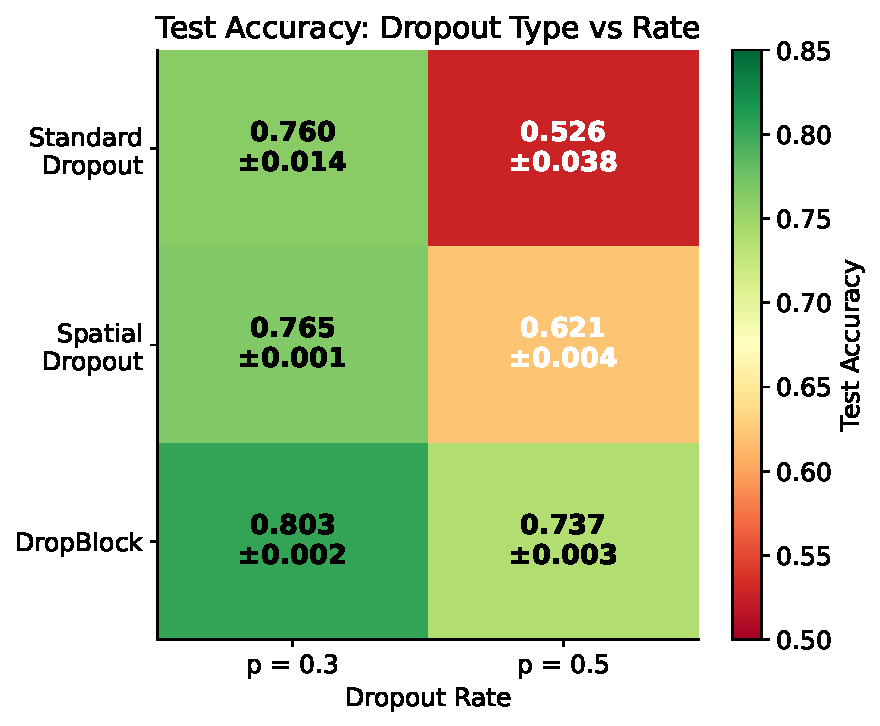
\includegraphics[width=0.6\textwidth]{analysis/figures/type_vs_rate_heatmap.pdf}
\caption{Test accuracy by dropout type and rate. DropBlock is the most robust to higher dropout rates, while standard dropout is most sensitive.}
\label{fig:heatmap}
\end{figure}

At a fixed rate of 0.3, the type effect is 4.3 percentage points (DropBlock 80.3\% vs.\ Standard 76.0\%). At a fixed rate of 0.5, the type effect grows to 21.1 percentage points (DropBlock 73.7\% vs.\ Standard 52.6\%). This confirms that dropout type matters, and its importance increases at higher dropout rates.

\subsection{Training Dynamics}

Figure~\ref{fig:training-curves} shows training loss and validation accuracy curves across all conditions.

\begin{figure}[t]
\centering
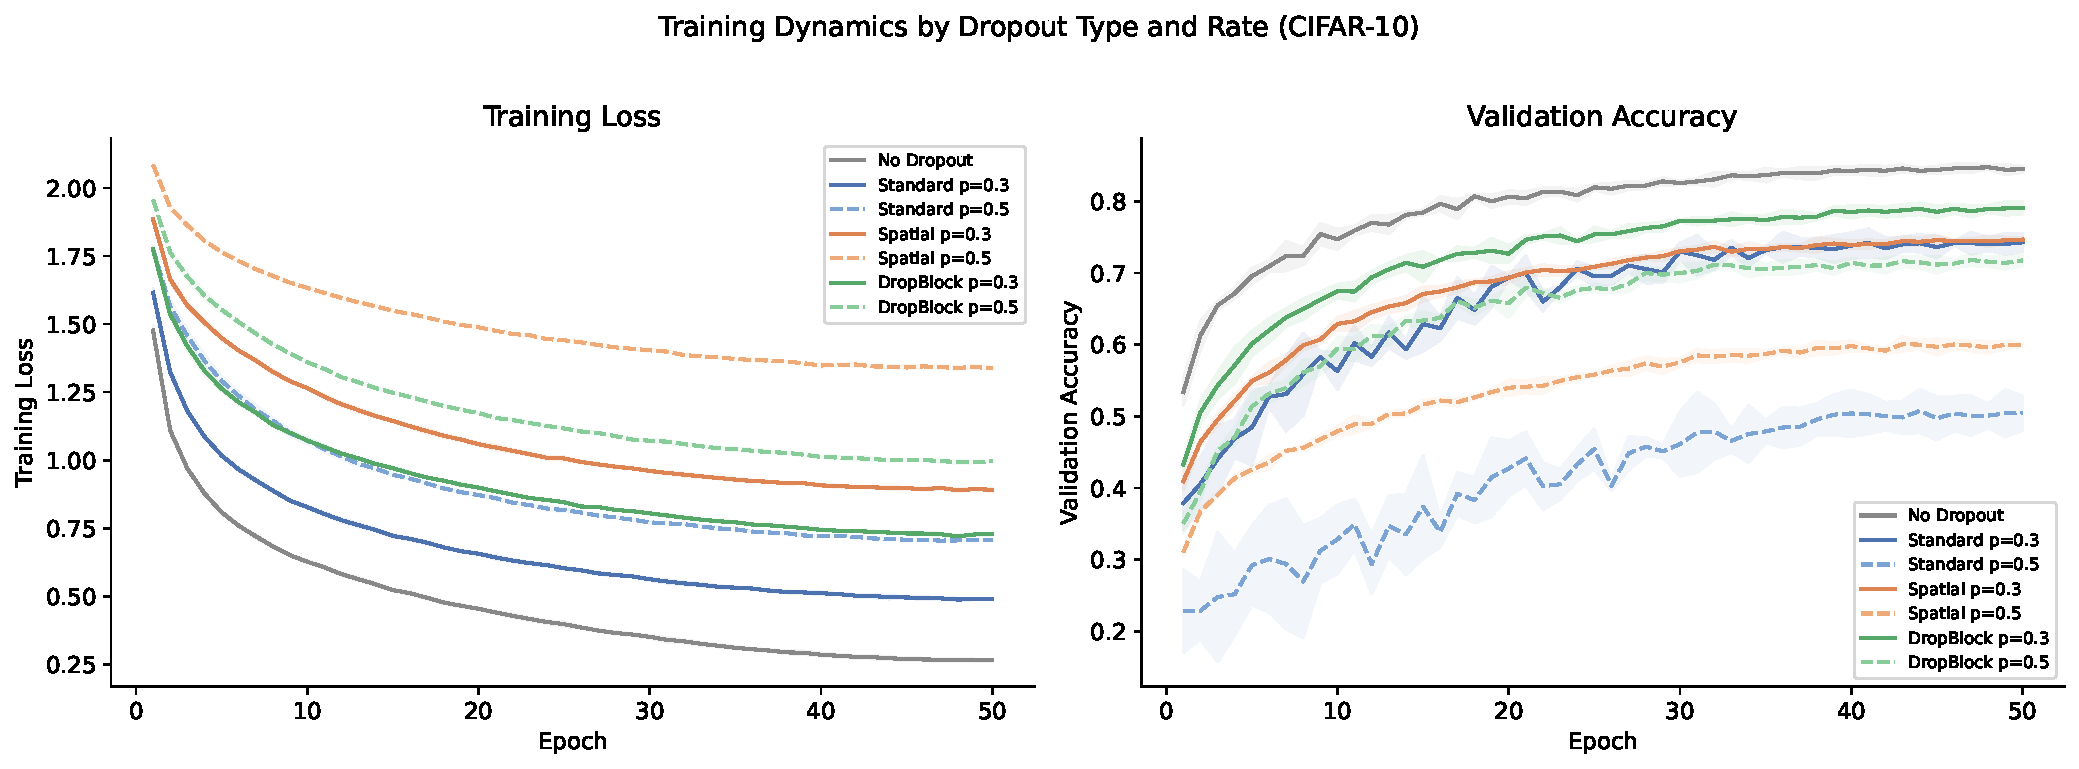
\includegraphics[width=\textwidth]{analysis/figures/training_curves.pdf}
\caption{Training loss (left) and validation accuracy (right) over 50 epochs. Higher dropout rates significantly slow convergence. Standard dropout at $p{=}0.5$ shows the slowest convergence and highest residual loss.}
\label{fig:training-curves}
\end{figure}

The no-dropout baseline converges fastest, reaching 80\% validation accuracy by epoch 17. DropBlock at $p{=}0.3$ is the only dropout configuration to reach 80\% validation accuracy, doing so at epoch 49---nearly 3$\times$ slower. All other dropout configurations fail to reach 80\% within 50 epochs.

\subsection{Generalization Gap Analysis}

Figure~\ref{fig:gen-gap} reveals a striking qualitative difference between dropout types. The generalization gap (train accuracy minus validation accuracy) shows two distinct behaviors:

\begin{figure}[t]
\centering
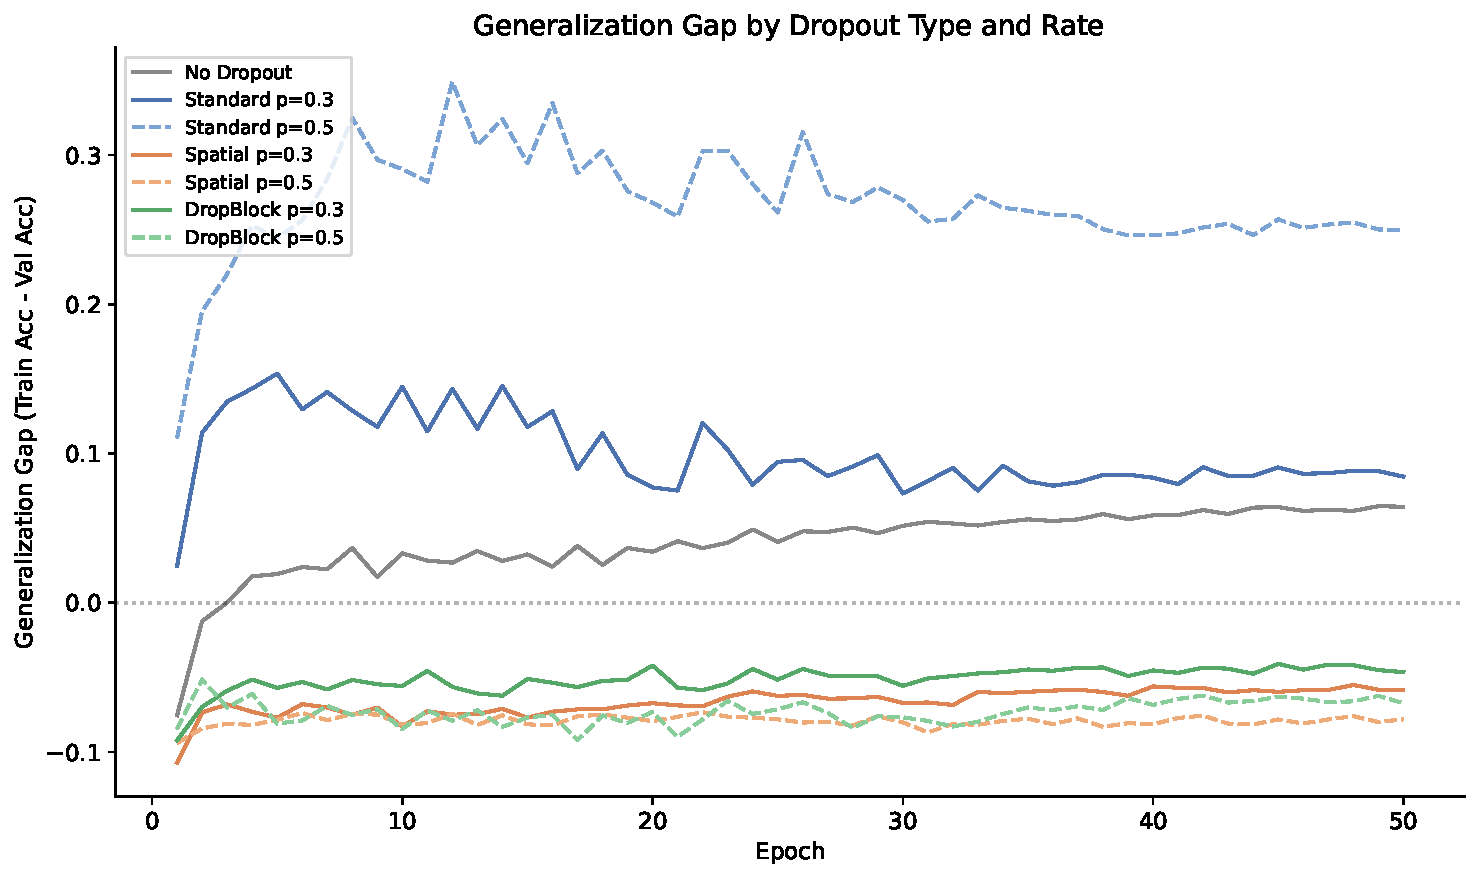
\includegraphics[width=0.8\textwidth]{analysis/figures/generalization_gap.pdf}
\caption{Generalization gap over training. Standard dropout shows positive gap (overfitting), while Spatial and DropBlock show negative gap (underfitting). Standard $p{=}0.5$ has the largest positive gap ($\sim$0.25), indicating it prevents the model from learning effectively.}
\label{fig:gen-gap}
\end{figure}

\begin{itemize}
    \item \textbf{Standard dropout} produces a \emph{positive} generalization gap (+0.08 at $p{=}0.3$, +0.25 at $p{=}0.5$), meaning training accuracy exceeds validation accuracy. At $p{=}0.5$, this gap is enormous---the model learns training patterns that do not generalize, likely because element-wise dropout in convolutional layers disrupts spatial features without providing meaningful regularization.
    \item \textbf{Spatial and DropBlock} produce \emph{negative} generalization gaps ($-$0.05 to $-$0.08), meaning validation accuracy \emph{exceeds} training accuracy. This occurs because these structured dropout types genuinely regularize the model---at test time, with dropout disabled, the full model performs better than the noisy training-time sub-models.
\end{itemize}

This negative gap for structured dropout methods is a healthy sign of effective regularization, contrasting sharply with standard dropout's behavior.

\section{Discussion}

\paragraph{Why does the no-dropout baseline win?}
All dropout configurations underperform the no-dropout baseline (85.7\%) at 50 epochs. We attribute this to two factors: (1) the model is relatively small (3 conv blocks, $\sim$200K parameters), limiting its tendency to overfit on CIFAR-10 within 50 epochs; (2) batch normalization already provides implicit regularization~\citep{krizhevsky2012}. With more training epochs or a larger model, the regularization benefit of dropout would likely emerge, especially for DropBlock.

\paragraph{Why is standard dropout so bad at $p{=}0.5$?}
Standard element-wise dropout at $p{=}0.5$ zeros half of all feature map elements independently. Because neighboring pixels carry correlated information, the remaining pixels partially compensate, but the noise injection is strong enough to severely disrupt learned spatial patterns. The model cannot learn coherent spatial features during training, leading to the large positive generalization gap. In contrast, DropBlock at $p{=}0.5$ drops contiguous regions, which provides a cleaner training signal by forcing the network to learn from different spatial regions rather than noisy corruptions of the same regions.

\paragraph{Practical recommendations.}
Based on our results:
\begin{enumerate}
    \item If using dropout in CNN convolutional layers, use DropBlock or Spatial dropout, not standard element-wise dropout.
    \item Use lower dropout rates ($p \leq 0.3$) for convolutional layers, regardless of dropout type.
    \item For small CNNs with batch normalization, consider whether dropout is needed at all---the no-dropout baseline may suffice.
\end{enumerate}

\paragraph{Limitations.}
Our study uses a single simple CNN architecture on CIFAR-10. Results may differ for deeper architectures (ResNets, DenseNets), larger datasets (ImageNet), or different training durations. The DropBlock block size ($b{=}3$) was not tuned; different block sizes may yield different results. We also did not explore the interaction between dropout and other regularization techniques (weight decay, data augmentation strength).

\section{Conclusion}

We presented a controlled factorial comparison of three dropout types (Standard, Spatial, DropBlock) at two rates (0.3, 0.5) on a simple CNN trained on CIFAR-10. Our key findings are:

\begin{enumerate}
    \item \textbf{Dropout type matters more than rate}, especially at higher dropout rates where DropBlock maintains reasonable performance while standard dropout degrades catastrophically.
    \item \textbf{DropBlock is the most robust dropout type} for convolutional layers, losing only 6.6pp when the rate increases from 0.3 to 0.5, compared to 23.4pp for standard dropout.
    \item \textbf{Structured dropout methods (Spatial, DropBlock) produce healthy negative generalization gaps}, while standard element-wise dropout produces pathological positive gaps in convolutional layers.
    \item \textbf{For small CNNs, dropout may not help within short training budgets}, as all dropout configurations underperformed the no-dropout baseline at 50 epochs.
\end{enumerate}

Future work should extend this comparison to deeper architectures and longer training schedules where dropout's regularization benefits are expected to be more pronounced.

\bibliography{paper}

\end{document}
